\chapter{Evaluation}~\label{cha:evaluation}
Once the application was deployed it had to be determined if the application met the requirements set out in the design phase. To do this the tests set out in Section~\ref{sec:test-design} were carried out.

\section{Primary Features}
These tests relate to the two primary feature tests set out in Section~\ref{sec:test-design}. As these features are fundamental to the application's core functionality, their implementation is critical in determining whether the project is a success. If the application failed to meet these criteria, it would be hard to consider the outcome a full success

\subsection{Album Scanning}
The album scanning mechanism consisted of two separate APIs, and the evaluation focuses on the accuracy of these two APIs as well as the effectiveness of the two methods used to identify albums, namely, using either the best guess from reverse image search results or extracted website titles.

To conduct the evaluation, fifteen albums were tested. For each album, six images were used as is shown in Table~\ref{tab:image-evaluation-examples}.
\ifshowappendix
Each used album is listed in Appendix~\ref{apd:test_albums}.
\fi

\begin{table} [H]
    \centering
    \renewcommand{\arraystretch}{1.5} % Adjust row height
    \setlength{\tabcolsep}{10pt}      % Adjust column spacing

    \begin{subtable}{0.48\textwidth}
        \centering
        \begin{tabular}{|m{2.5cm}|m{2.5cm}|}
            \hline
            \textbf{Image Type} & \textbf{Example} \\
            \hline
            Normal & 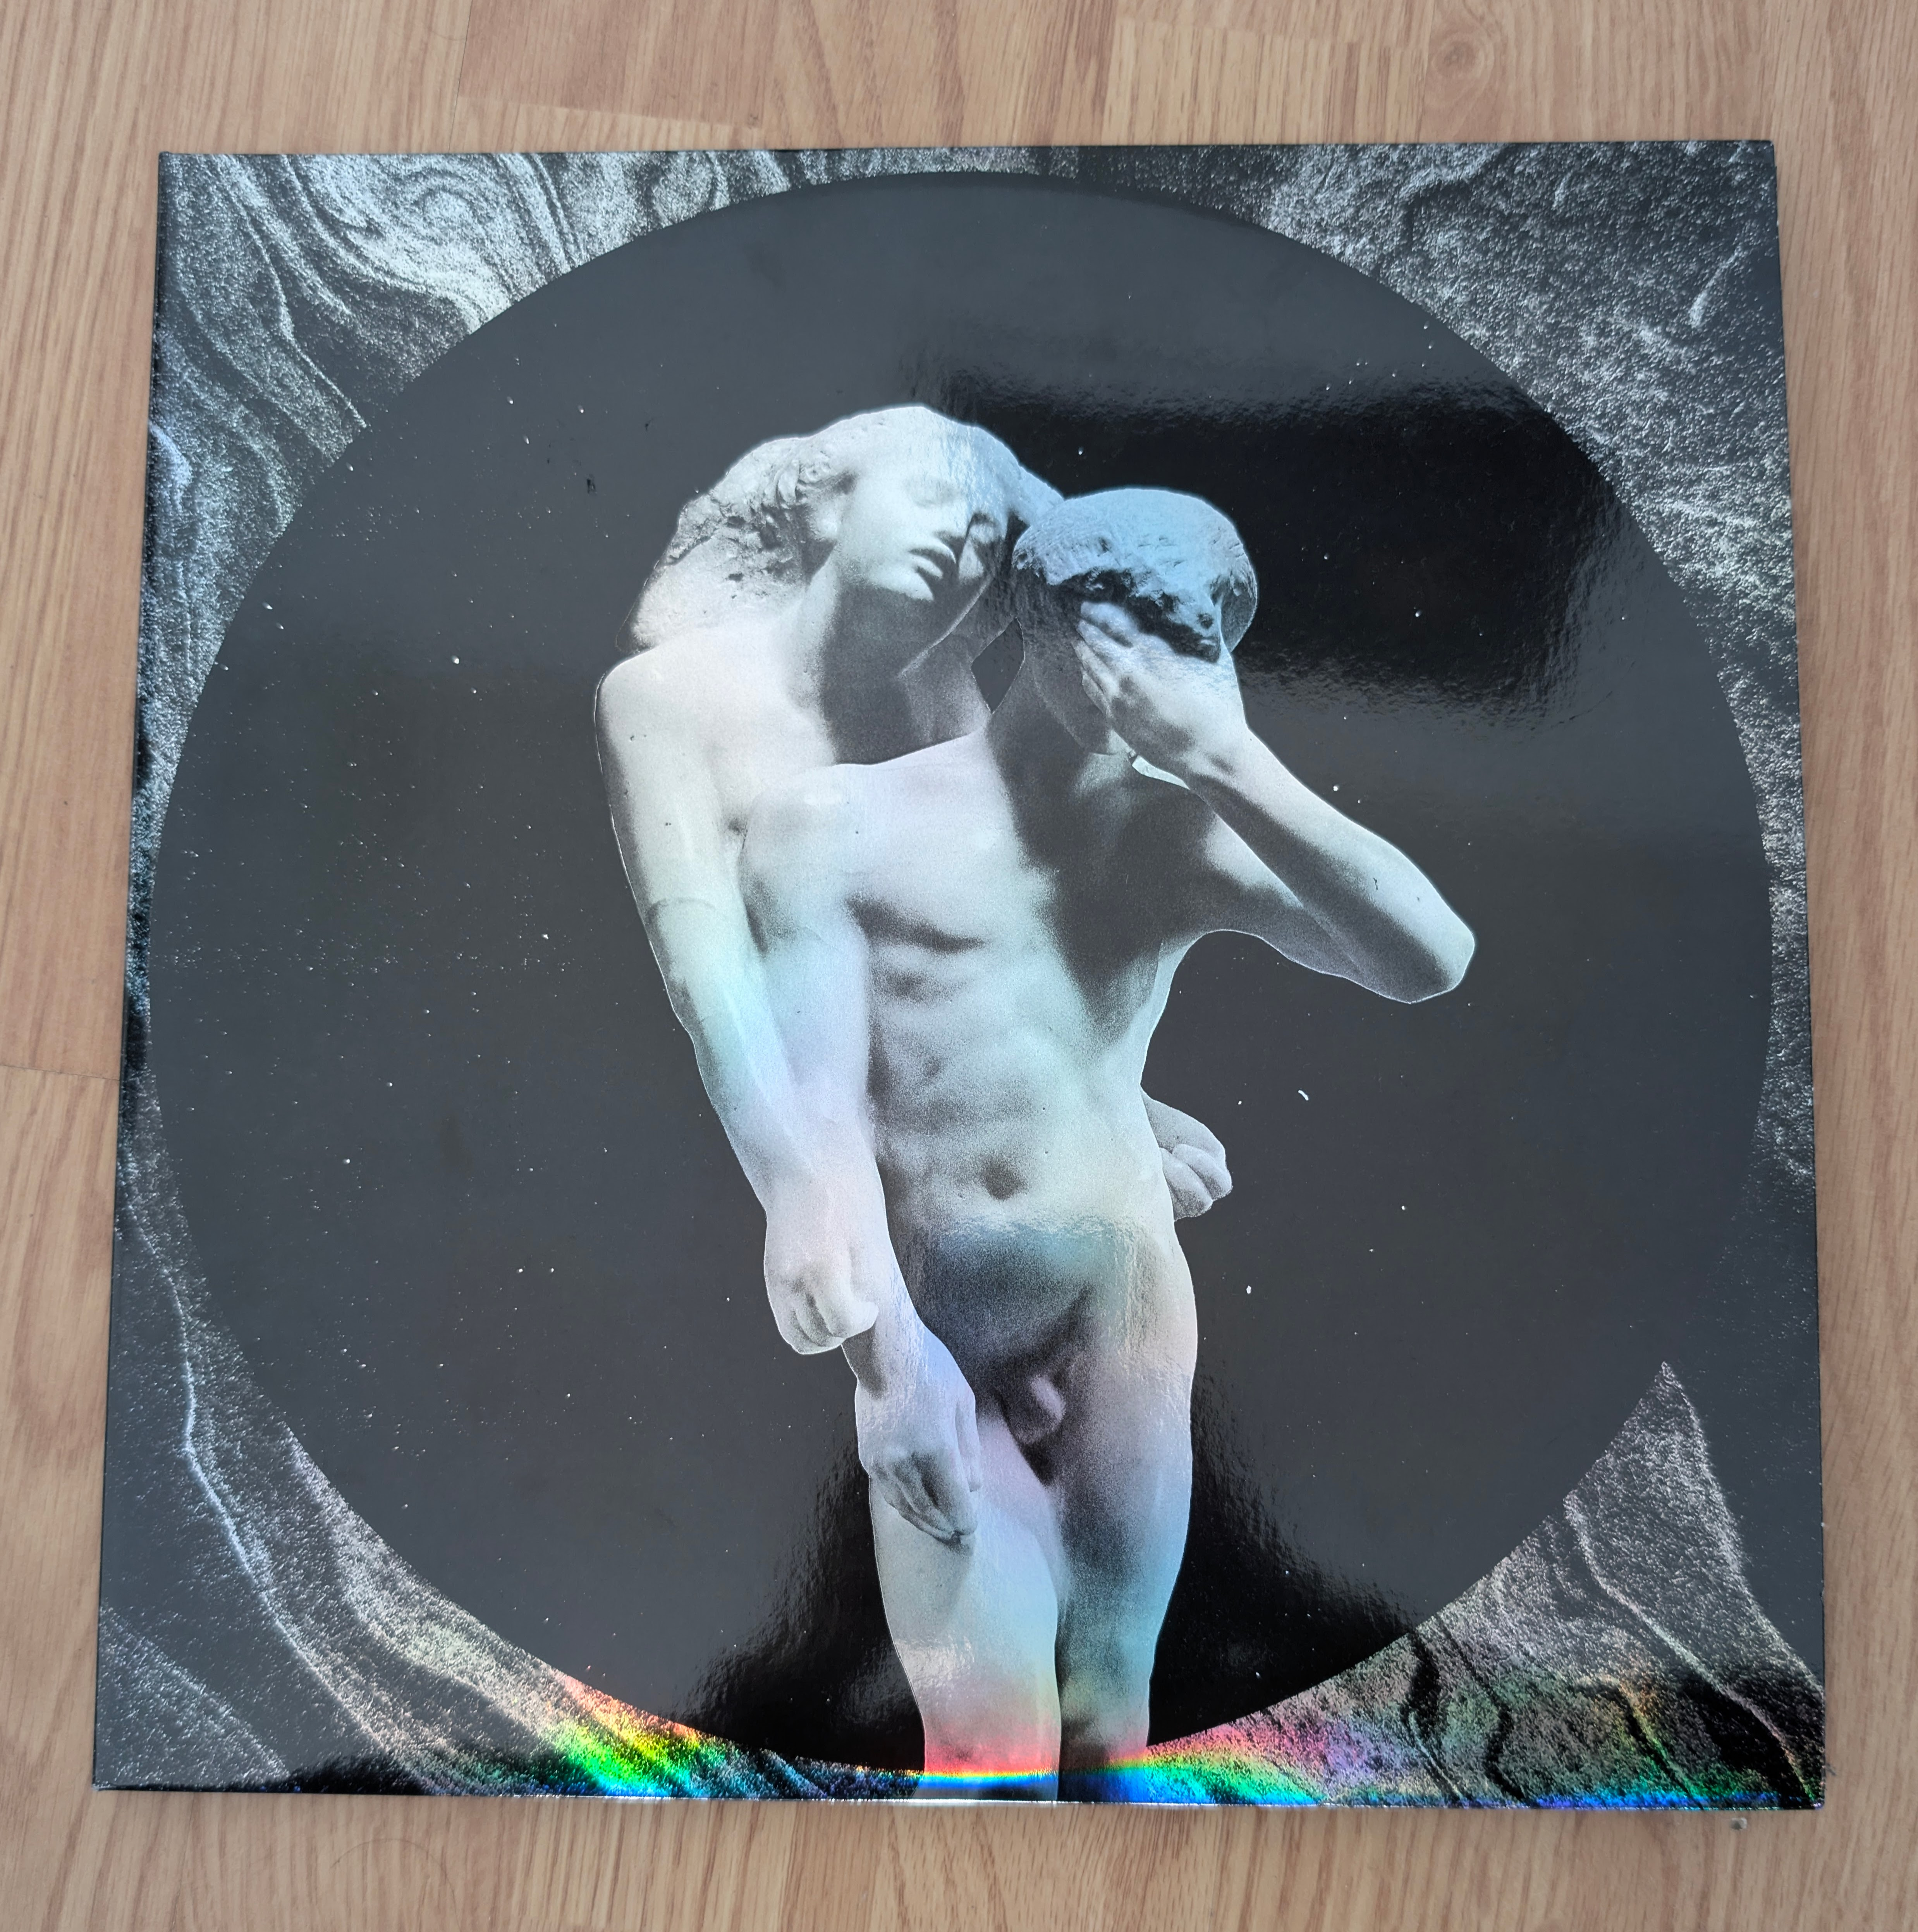
\includegraphics[width=2.5cm]{figures/test_albums/Reflektor.jpg} \\
            \hline
            Rotated $90$\textdegree & 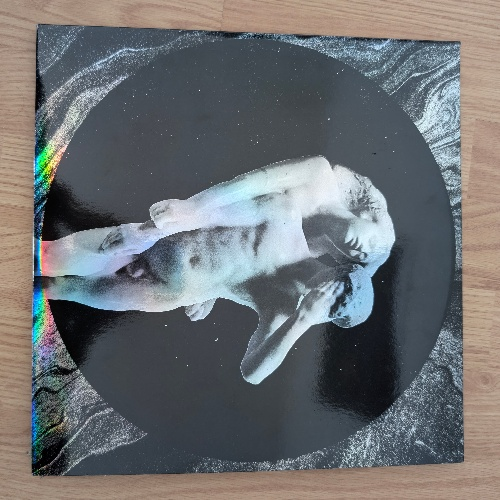
\includegraphics[width=2.5cm]{figures/test_albums/Reflektor_Rotated - 90.jpg} \\
            \hline
            Rotated $180$\textdegree & 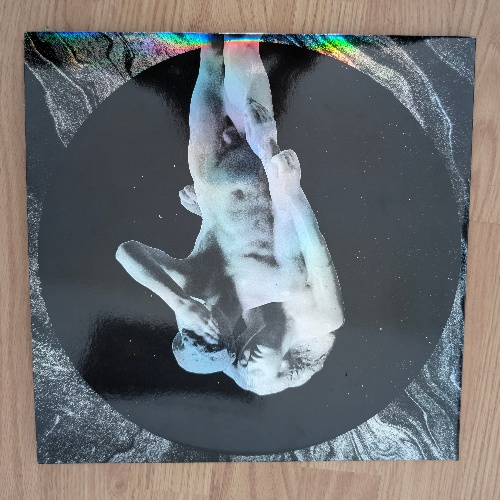
\includegraphics[width=2.5cm]{figures/test_albums/Reflektor_Rotated - 180.jpg} \\
            \hline
        \end{tabular}
    \end{subtable}
    \hfill
    \begin{subtable}{0.48\textwidth}
        \centering
        \begin{tabular}{|m{2.5cm}|m{2.5cm}|}
            \hline
            \textbf{Image Type} & \textbf{Example} \\
            \hline
            Rotated $270$\textdegree & 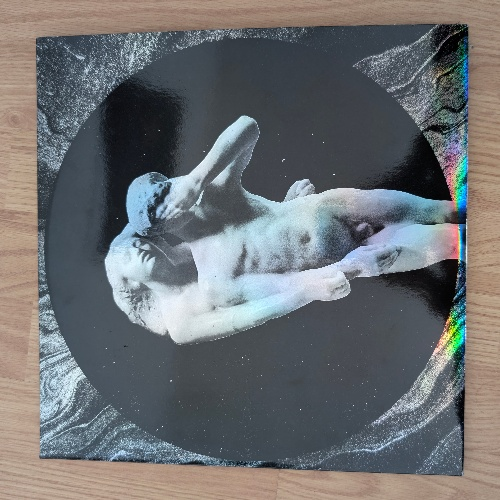
\includegraphics[width=2.5cm]{figures/test_albums/Reflektor_Rotated - 270.jpg} \\
            \hline
            Blurred & 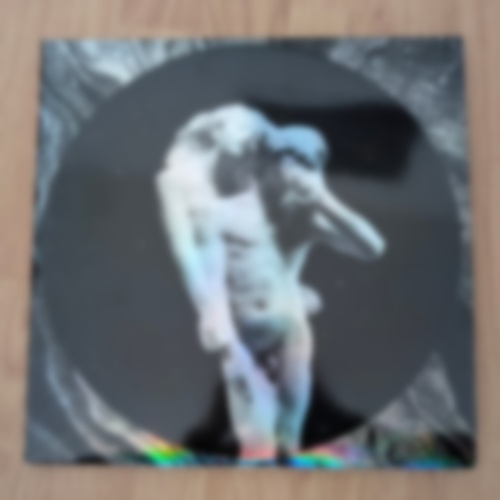
\includegraphics[width=2.5cm]{figures/test_albums/Reflektor_Blurred.jpg} \\
            \hline
            Scaled Down & 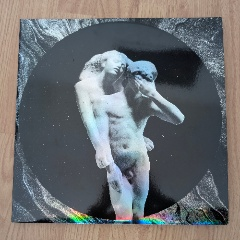
\includegraphics[width=2.5cm]{figures/test_albums/Reflektor_Scaled.jpg} \\
            \hline
        \end{tabular}
    \end{subtable}

    \caption{Example images used in the evaluation}
    \label{tab:image-evaluation-examples}
\end{table}

Self-taken images were used to ensure that the test cases were more representative of real user-uploaded images, this is opposed to using images already present on the internet which could be pre-indexed by the search engines.

The criteria for a pass were defined as follows:
\begin{itemize}
    \item For reverse image search, a result was considered correct if the exact album name appeared in the returned results.
    \item For the Spotify search, a result was deemed correct if the correct album was returned.
\end{itemize}

\subsubsection{Results}
The results are split into two sets:
\begin{itemize}
    \item Reverse Image Search Accuracy – Displayed in Figure~\ref{fig:album-scanning-results-ris}, this dataset evaluates the accuracy of the Google Reverse Image Search API. While this API functions as a black box as the application cannot affect its inner working, it is still valuable to evaluate how accurate it is in practice.
    \item Spotify Search Accuracy – Displayed in Figure~\ref{fig:album-scanning-results-spotify}, this dataset evaluates the accuracy of the Spotify Search API, considering only cases where the reverse image search correctly identified the album so the accuracy of the Spotify search could be isolated from the accuracy of the reverse image search.
\end{itemize}

\begin{figure} [H]
    \centering
    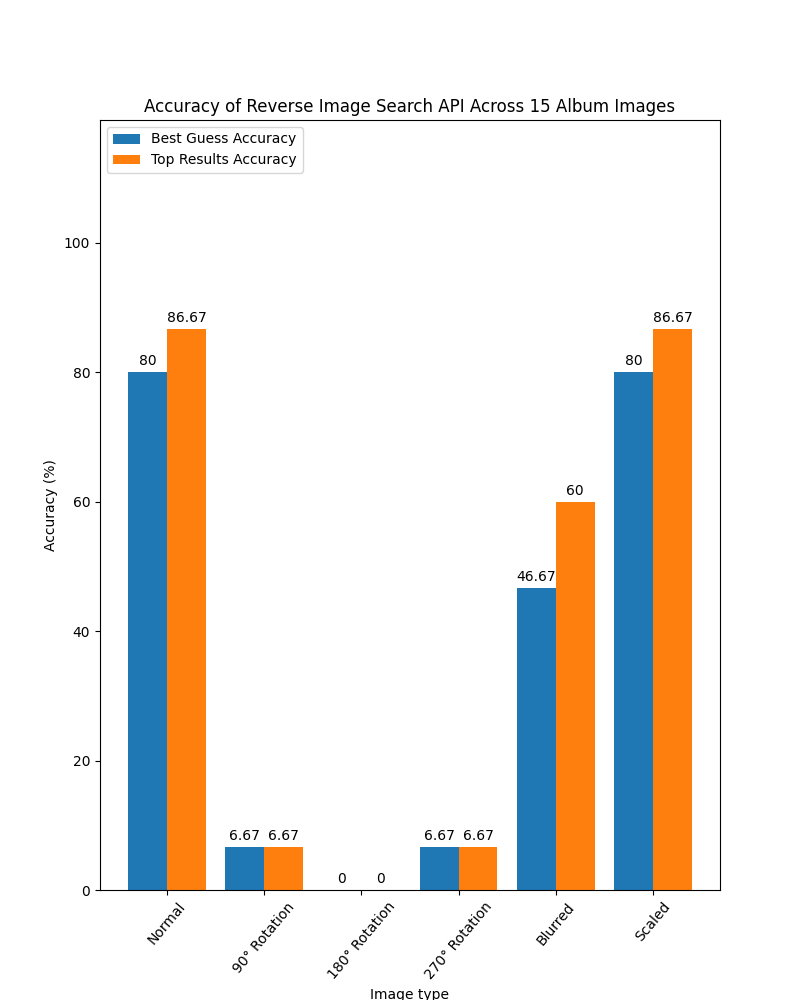
\includegraphics[width=0.65\textwidth]{figures/evaluation_graphs_ris.png}
    \caption{Accuracy of Reverse Image Search}
    \label{fig:album-scanning-results-ris}
\end{figure}

The results from the reverse image search did not meet expectations. While an accuracy of $95\%$ was targeted, the measured accuracy for images with no modification was significantly lower:
\begin{itemize}
    \item $80\%$ ($12$ out of $15$) accuracy when using the best guess from the reverse image search results.
    \item $86.67\%$ ($13$ our of $15$) accuracy when using website titles extracted from the search results.
\end{itemize}

Performance was particularly poor for rotated images, with only albums that had rotated artwork being correctly identified. The two examples of this in the test dataset are shown in Figures~\ref{fig:sos_rotated_90} and~\ref{fig:tih_rotated_270}.

\begin{figure} [H]
    \captionsetup{justification=centering}
    \centering
    \begin{subfigure}[t]{0.45\textwidth}
        \centering
        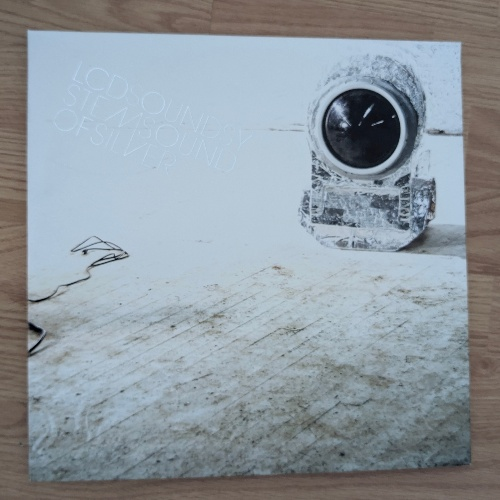
\includegraphics[width=0.45\textwidth]{figures/test_albums/Sound_Of_Silver_Rotated - 90.jpg}
        \caption{The only correct result for 90° rotation}
        \label{fig:sos_rotated_90}
    \end{subfigure}
    \begin{subfigure}[t]{0.45\textwidth}
        \centering
        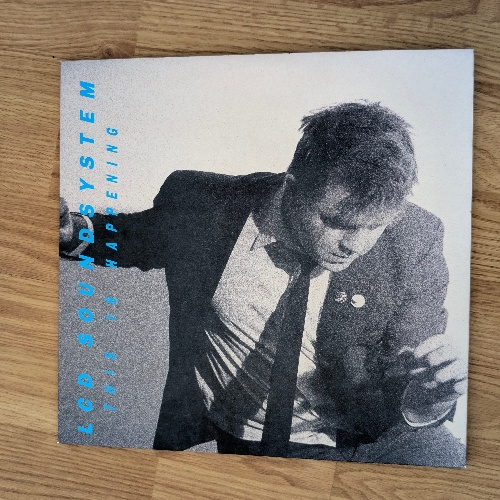
\includegraphics[width=0.45\textwidth]{figures/test_albums/This_Is_Happening_Rotated - 270.jpg}
        \caption{The only correct result for 270° rotation}
        \label{fig:tih_rotated_270}
    \end{subfigure}
\end{figure}

Despite the shortcomings of the reverse image search, the results indicate the scatter-shot approach, using website titles, was equally or more successful across all categories of images. This validates the choice to include it as it improves the overall chances of identification.

\begin{figure} [H]
    \centering
    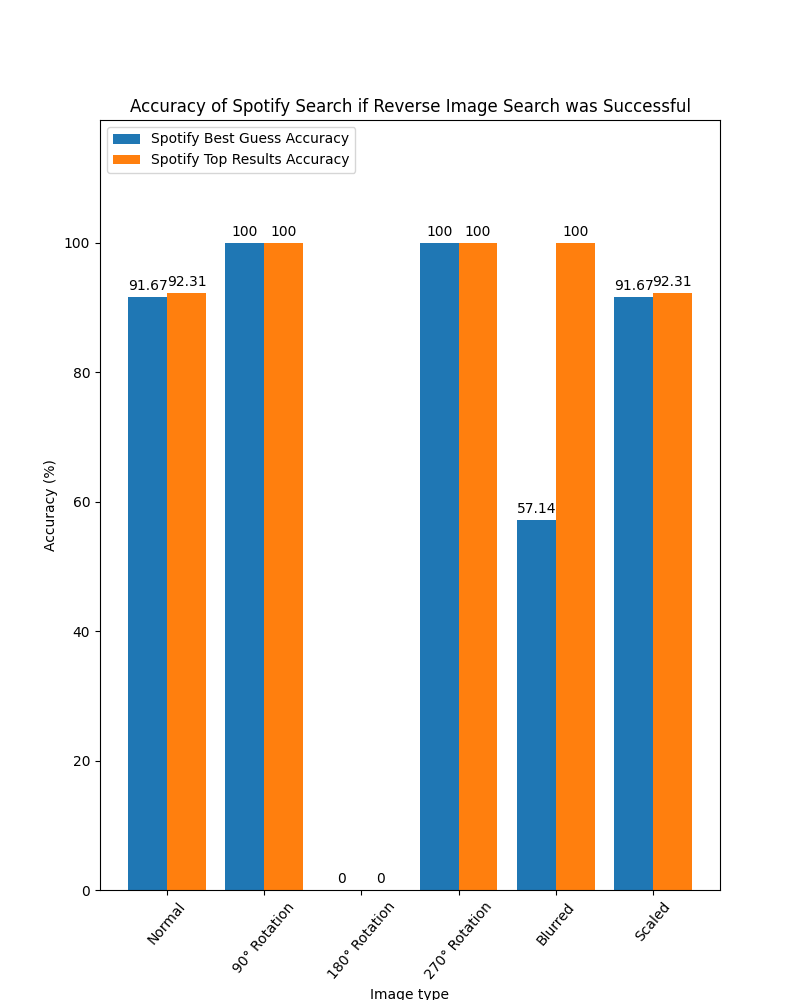
\includegraphics[width=0.65\textwidth]{figures/evaluation_graphs_spotify.png}
    \caption{Accuracy of Spotify Search}
    \label{fig:album-scanning-results-spotify}
\end{figure}

The results from the Spotify search API demonstrated strong performance. When provided with a correct reverse image search result, the Spotify search successfully identified the correct album in:

\begin{itemize}
    \item $91.67\%$ (11 out of 12 cases) for best guess searches.
    \item $92.31\%$ (12 out of 13 cases) for website title-based searches.
\end{itemize}

These results indicate that the chosen method, directly using reverse image search outputs with no processing as inputs for the Spotify search API, was broadly effective, even though it did not achieve the target $95\%$ accuracy.

\subsubsection{Key Takeaways}
The primary limiting factor in the system's accuracy is the accuracy of the reverse image search API. So by extension, any changes to improve this accuracy should focus on enhancing this APIs accuracy.

Since the Google reverse image search API is treated as a black box, direct improvements to its internal processing are not possible. This leaves only one option to improve its accuracy, input refinement. Two possible approaches include:

\begin{itemize}
    \item Pre-processing the image – Applying pre-processing techniques to remove backgrounds before passing the image to the API for example segmentation where the background of the image is removed automatically %[TODO: Add reference to segmentation potentially]
    \item User-assisted cropping – Prompting users to manually crop the image, ensuring only the album cover is submitted for identification
\end{itemize}

Though these methods may improve accuracy, the first could introduce additional UI elements making the system more complex from a user perspective. The second may increase the time required to scan an album. Therefore, any enhancements should be carefully evaluated to balance accuracy improvements with user experience.

It should also be noted that the sample size for testing was relatively small, with only fifteen albums evaluated. As a result, the accuracy figures obtained may not be fully representative of the system's performance on a larger and more diverse dataset. For example, it is likely less popular albums are less likely to be identified, and more popular albums are more likely to be identified. Testing with a broader selection of albums would be necessary to obtain a more comprehensive assessment of the system’s accuracy and limitations.

\subsection{Album Playback}
This test aimed to verify that the music playback functionality operated as intended. The most effective approach was to evaluate the application from a user perspective, simulating real-world usage by using it to listen to whole albums, ensuring that playback functioned correctly.
\ifshowappendix
Testing was conducted using a subset of five of the albums listed in Appendix~\ref{apd:test_albums}.
\fi

\subsubsection{Results}
The results of this test were entirely positive. All selected albums played from start to finish without issues. Additionally, the music controls, including play, pause, and skip—functioned as expected, and album artwork and track information were displayed correctly throughout playback as the tracks changed.

\section{User Interface}
The survey described in Section~\ref{sec:test-design} was used to evaluate the user interface. In total [TODO: Add number] participants completed the survey.

\subsection{Results}
[TODO: Add results from survey]

\subsection{Participants}
Ideally, the user interface evaluation would have been conducted with a large and diverse user base to gather feedback from individuals with varying levels of technical expertise. However, this was beyond the scope of the current evaluation, and instead, a smaller sample group was used.

It is important to acknowledge the potential biases in the participant selection. The sample group consisted primarily of friends and family, many of whom were computer science students. As a result, the participants may have been more familiar with the technology than the average user and could also have been predisposed to providing more favourable reviews as not to disappoint the creator of the application. Because of this, while the survey provides useful insights, the findings may not be fully representative of a broader user base.

\section{Development Practices}
The development practices were evaluated based on the tests set out in Section~\ref{sec:test-design}. A pass was defined as meeting the verification specified.

\subsection{Testing And Test Coverage}
All tests defined in all test cases were executed and all passed as was expected as this was enforced by automated actions before code could be merged into the main branch of the repository.

Test coverage was measured using pytest-cov for the backend and Vitest for the frontend. The target was set at $95\%$ line and branch coverage for both the frontend and backend. The results are shown in Table~\ref{tab:test-coverage-results}.
\begin{table} [H]
    \centering
    \begin{tabular}{|m{3cm}|m{3cm}|}
        \hline
        \textbf{Component} & \textbf{Coverage} \\
        \hline
        Backend & $100\%$ \\
        \hline
        Frontend & $95\%$ \\
        \hline
    \end{tabular}
    \caption{Test Coverage Results}
    \label{tab:test-coverage-results}
\end{table}

The backend achieved full coverage with all lines and branches tested. The frontend achieved $95\%$ coverage, which whilst meeting the target is likely a result of the inexperience of the developer in frontend development with many changes needed even after the tests were originally defined.

Code coverage though did cover all important aspects of the application and as such can be considered a success.
\ifshowappendix
A full list of the tests can be found in Appendix~\ref{apd:testcases}.
\fi

\subsection{Code Quality}
The code quality objectives of enforcing formatting and linting were successfully achieved through the use of pre-commit hooks. This ensured that all code committed to the repository adhered to established formatting and linting rules.

Though this approach was effective for a single developer, in hindsight, it may not have been ideal for team-based development because pre-commit hooks require each developer to manually install them. A much more robust approach would have been to enforce these rules using GitHub Actions that run on pull requests. This could either format the code itself or reject the pull request if the code did not meet the required standards, forcing the developer to run the formatting and linting tools locally before pushing their changes achieving the same goal as the pre-commit hooks.

\subsection{Automated Deployment and Dependency Management}
The automated deployment process was successfully implemented. Once configured on Google Cloud Run, the application could be rebuilt and deployed automatically whenever a new tag was pushed to the repository.

Similarly, automated dependency management was effectively set up using Dependabot, with checks for updates running every week. Over the course of development, $110$ pull requests were generated for dependency updates, with only three requiring manual intervention, primarily due to breaking changes. It is of note that none of the changes that passed all tests actually resulted in breaking changes to the application, suggesting that the testing system in place was effective in verifying functionality after each update.
